\documentclass{standalone}
\usepackage{tikz}
\usetikzlibrary{patterns, positioning}
\usepackage[sfdefault]{ClearSans} %% option 'sfdefault' activates Clear Sans as the default text font
\usepackage[T1]{fontenc}

\begin{document}
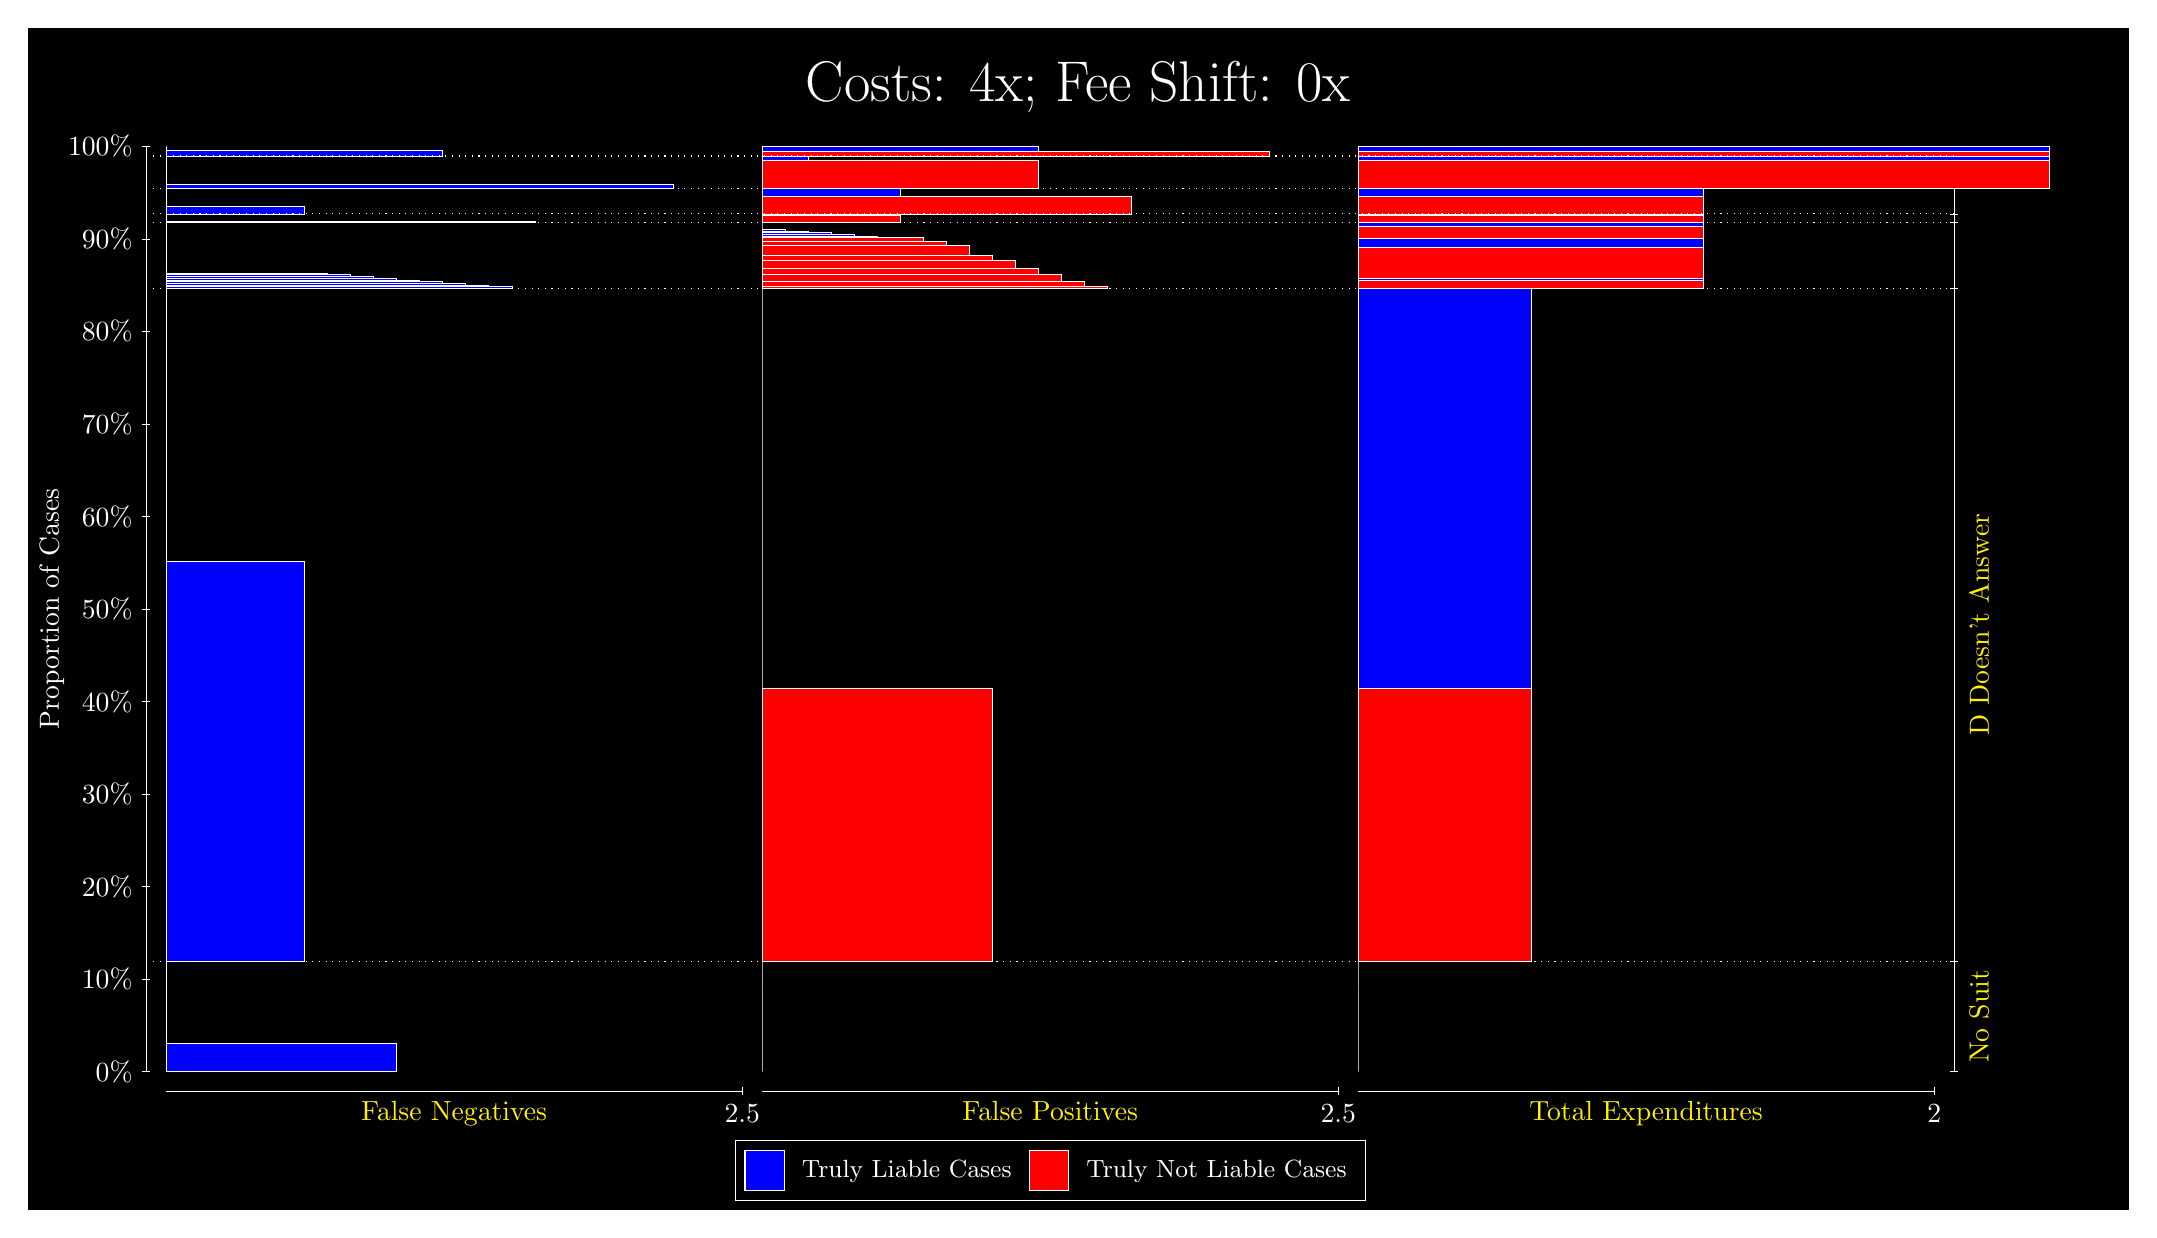
\begin{tikzpicture}
\draw[fill=black] (0,0) rectangle (26.667,15);
\draw[text=white] (0,13.5) rectangle (26.667,15) node[midway] {\huge Costs: 4x; Fee Shift: 0x};
\draw[white, very thin] (1.5,1.75) -- (1.5,13.5);
\node[rotate=90, text=white, anchor=center] at (0.3, 7.625) {Proportion of Cases};
\draw[white, very thin] (1.45,1.75) -- (1.55,1.75);
\node[text=white, anchor=east] at (1.45, 1.75) {0\%};
\draw[white, very thin] (1.45,2.925) -- (1.55,2.925);
\node[text=white, anchor=east] at (1.45, 2.925) {10\%};
\draw[white, very thin] (1.45,4.1) -- (1.55,4.1);
\node[text=white, anchor=east] at (1.45, 4.1) {20\%};
\draw[white, very thin] (1.45,5.275) -- (1.55,5.275);
\node[text=white, anchor=east] at (1.45, 5.275) {30\%};
\draw[white, very thin] (1.45,6.45) -- (1.55,6.45);
\node[text=white, anchor=east] at (1.45, 6.45) {40\%};
\draw[white, very thin] (1.45,7.625) -- (1.55,7.625);
\node[text=white, anchor=east] at (1.45, 7.625) {50\%};
\draw[white, very thin] (1.45,8.8) -- (1.55,8.8);
\node[text=white, anchor=east] at (1.45, 8.8) {60\%};
\draw[white, very thin] (1.45,9.975) -- (1.55,9.975);
\node[text=white, anchor=east] at (1.45, 9.975) {70\%};
\draw[white, very thin] (1.45,11.15) -- (1.55,11.15);
\node[text=white, anchor=east] at (1.45, 11.15) {80\%};
\draw[white, very thin] (1.45,12.325) -- (1.55,12.325);
\node[text=white, anchor=east] at (1.45, 12.325) {90\%};
\draw[white, very thin] (1.45,13.5) -- (1.55,13.5);
\node[text=white, anchor=east] at (1.45, 13.5) {100\%};

\draw[white, very thin] (24.457,1.75) -- (24.457,13.5);
\draw[white, very thin] (24.407,1.75) -- (24.507,1.75);
\node[anchor=west] at (24.407, 1.75) {};
\draw[white, very thin] (24.407,3.1524) -- (24.507,3.1524);
\node[anchor=west] at (24.407, 3.1524) {};
\draw[white, very thin] (24.407,11.698) -- (24.507,11.698);
\node[anchor=west] at (24.407, 11.698) {};
\draw[white, very thin] (24.407,12.532) -- (24.507,12.532);
\node[anchor=west] at (24.407, 12.532) {};
\draw[white, very thin] (24.407,12.642) -- (24.507,12.642);
\node[anchor=west] at (24.407, 12.642) {};
\draw[white, very thin] (24.407,12.962) -- (24.507,12.962);
\node[anchor=west] at (24.407, 12.962) {};
\draw[white, very thin] (24.407,13.377) -- (24.507,13.377);
\node[anchor=west] at (24.407, 13.377) {};
\draw[white, very thin] (24.407,13.5) -- (24.507,13.5);
\node[anchor=west] at (24.407, 13.5) {};

\draw[white, very thin, fill=blue] (1.75,1.75) rectangle (4.6775,2.1125);
\draw[white, very thin, fill=red] (1.75,2.1125) rectangle (1.75,3.1524);
\draw[white, very thin, fill=blue] (1.75,3.1524) rectangle (3.5065,8.2327);
\draw[white, very thin, fill=red] (1.75,8.2327) rectangle (1.75,11.698);
\draw[white, very thin, fill=blue] (1.75,11.698) rectangle (6.1413,11.717);
\draw[white, very thin, fill=blue] (1.75,11.717) rectangle (5.8486,11.733);
\draw[white, very thin, fill=blue] (1.75,11.733) rectangle (5.5558,11.761);
\draw[white, very thin, fill=blue] (1.75,11.761) rectangle (5.2631,11.78);
\draw[white, very thin, fill=blue] (1.75,11.78) rectangle (4.9703,11.804);
\draw[white, very thin, fill=blue] (1.75,11.804) rectangle (4.6775,11.82);
\draw[white, very thin, fill=blue] (1.75,11.82) rectangle (4.3848,11.848);
\draw[white, very thin, fill=blue] (1.75,11.848) rectangle (4.092,11.87);
\draw[white, very thin, fill=blue] (1.75,11.87) rectangle (3.7993,11.888);
\draw[white, very thin, fill=red] (1.75,11.888) rectangle (1.75,12.532);
\draw[white, very thin, fill=blue] (1.75,12.532) rectangle (6.4341,12.549);
\draw[white, very thin, fill=red] (1.75,12.549) rectangle (1.75,12.642);
\draw[white, very thin, fill=blue] (1.75,12.642) rectangle (3.5065,12.743);
\draw[white, very thin, fill=red] (1.75,12.743) rectangle (1.75,12.962);
\draw[white, very thin, fill=blue] (1.75,12.962) rectangle (8.1906,13.018);
\draw[white, very thin, fill=red] (1.75,13.018) rectangle (1.75,13.377);
\draw[white, very thin, fill=blue] (1.75,13.377) rectangle (5.2631,13.445);
\draw[white, very thin, fill=red] (1.75,13.445) rectangle (1.75,13.5);
\draw[white, very thin, fill=red] (9.3189,1.75) rectangle (9.3189,2.7898);
\draw[white, very thin, fill=blue] (9.3189,2.7898) rectangle (9.3189,3.1524);
\draw[white, very thin, fill=red] (9.3189,3.1524) rectangle (12.246,6.618);
\draw[white, very thin, fill=blue] (9.3189,6.618) rectangle (9.3189,11.698);
\draw[white, very thin, fill=red] (9.3189,11.698) rectangle (13.71,11.728);
\draw[white, very thin, fill=red] (9.3189,11.728) rectangle (13.417,11.783);
\draw[white, very thin, fill=red] (9.3189,11.783) rectangle (13.125,11.872);
\draw[white, very thin, fill=red] (9.3189,11.872) rectangle (12.832,11.949);
\draw[white, very thin, fill=red] (9.3189,11.949) rectangle (12.539,12.05);
\draw[white, very thin, fill=red] (9.3189,12.05) rectangle (12.246,12.118);
\draw[white, very thin, fill=red] (9.3189,12.118) rectangle (11.954,12.237);
\draw[white, very thin, fill=red] (9.3189,12.237) rectangle (11.661,12.291);
\draw[white, very thin, fill=red] (9.3189,12.291) rectangle (11.368,12.343);
\draw[white, very thin, fill=blue] (9.3189,12.343) rectangle (10.783,12.361);
\draw[white, very thin, fill=blue] (9.3189,12.361) rectangle (10.49,12.383);
\draw[white, very thin, fill=blue] (9.3189,12.383) rectangle (10.197,12.411);
\draw[white, very thin, fill=blue] (9.3189,12.411) rectangle (9.9044,12.426);
\draw[white, very thin, fill=blue] (9.3189,12.426) rectangle (9.6116,12.451);
\draw[white, very thin, fill=blue] (9.3189,12.451) rectangle (9.3189,12.532);
\draw[white, very thin, fill=red] (9.3189,12.532) rectangle (11.075,12.626);
\draw[white, very thin, fill=blue] (9.3189,12.626) rectangle (9.3189,12.642);
\draw[white, very thin, fill=red] (9.3189,12.642) rectangle (14.003,12.861);
\draw[white, very thin, fill=blue] (9.3189,12.861) rectangle (11.075,12.962);
\draw[white, very thin, fill=red] (9.3189,12.962) rectangle (12.832,13.32);
\draw[white, very thin, fill=blue] (9.3189,13.32) rectangle (9.9044,13.377);
\draw[white, very thin, fill=red] (9.3189,13.377) rectangle (15.759,13.431);
\draw[white, very thin, fill=blue] (9.3189,13.431) rectangle (12.832,13.5);
\draw[white, very thin, fill=red] (16.888,1.75) rectangle (16.888,2.7898);
\draw[white, very thin, fill=blue] (16.888,2.7898) rectangle (16.888,3.1524);
\draw[white, very thin, fill=red] (16.888,3.1524) rectangle (19.083,6.618);
\draw[white, very thin, fill=blue] (16.888,6.618) rectangle (19.083,11.698);
\draw[white, very thin, fill=red] (16.888,11.698) rectangle (21.279,11.8);
\draw[white, very thin, fill=blue] (16.888,11.8) rectangle (21.279,11.825);
\draw[white, very thin, fill=red] (16.888,11.825) rectangle (21.279,12.223);
\draw[white, very thin, fill=blue] (16.888,12.223) rectangle (21.279,12.338);
\draw[white, very thin, fill=red] (16.888,12.338) rectangle (21.279,12.482);
\draw[white, very thin, fill=blue] (16.888,12.482) rectangle (21.279,12.532);
\draw[white, very thin, fill=red] (16.888,12.532) rectangle (21.279,12.626);
\draw[white, very thin, fill=blue] (16.888,12.626) rectangle (21.279,12.642);
\draw[white, very thin, fill=red] (16.888,12.642) rectangle (21.279,12.861);
\draw[white, very thin, fill=blue] (16.888,12.861) rectangle (21.279,12.962);
\draw[white, very thin, fill=red] (16.888,12.962) rectangle (25.67,13.32);
\draw[white, very thin, fill=blue] (16.888,13.32) rectangle (25.67,13.377);
\draw[white, very thin, fill=red] (16.888,13.377) rectangle (25.67,13.431);
\draw[white, very thin, fill=blue] (16.888,13.431) rectangle (25.67,13.5);
\draw[white, dotted] (1.5,3.1524) -- (24.457,3.1524);
\draw[white, dotted] (1.5,11.698) -- (24.457,11.698);
\draw[white, dotted] (1.5,12.532) -- (24.457,12.532);
\draw[white, dotted] (1.5,12.642) -- (24.457,12.642);
\draw[white, dotted] (1.5,12.962) -- (24.457,12.962);
\draw[white, dotted] (1.5,13.377) -- (24.457,13.377);
\draw[white, very thin] (1.75,1.5) -- (9.0689,1.5);
\node[text=yellow, anchor=north] at (5.4094, 1.5) {False Negatives};
\draw[white, very thin] (9.0689,1.45) -- (9.0689,1.55);
\node[text=white, anchor=north] at (9.0689, 1.45) {2.5};

\draw[white, very thin] (9.3189,1.5) -- (16.638,1.5);
\node[text=yellow, anchor=north] at (12.978, 1.5) {False Positives};
\draw[white, very thin] (16.638,1.45) -- (16.638,1.55);
\node[text=white, anchor=north] at (16.638, 1.45) {2.5};

\draw[white, very thin] (16.888,1.5) -- (24.207,1.5);
\node[text=yellow, anchor=north] at (20.547, 1.5) {Total Expenditures};
\draw[white, very thin] (24.207,1.45) -- (24.207,1.55);
\node[text=white, anchor=north] at (24.207, 1.45) {2};

\node[text=yellow, centered, rotate=90] at (24.777, 2.4512) {No Suit};
\node[text=yellow, centered, rotate=90] at (24.777, 7.4254) {D Doesn't Answer};






\draw (12.978300999999998,1.5) node[draw=none] (baseCoordinate) {};
\begin{scope}[align=center]
        \matrix[scale=0.5, draw=white, below=0.5cm of baseCoordinate, nodes={draw}, column sep=0.1cm]{
            \node[rectangle, draw, minimum width=0.5cm, minimum height=0.5cm, fill=blue] {}; &
            \node[draw=none, font=\small, text=white] (B) {Truly Liable Cases}; &
            \node[rectangle, draw, minimum width=0.5cm, minimum height=0.5cm, fill=red] {}; &
            \node[draw=none, font=\small, text=white] (B) {Truly Not Liable Cases}; \\
            };
\end{scope}

\end{tikzpicture}
\end{document}